% A Gaussian surface around a point charge.
%
% Pulled in with \tikzfig{gauss-sphere.tex}. This file is a fragment, not a
% document -- it contains exactly one tikzpicture and no preamble, so it is
% typeset by whatever document \input's it and inherits that document's fonts.
% Keeping figures as their own files means they can be reused across chapters.
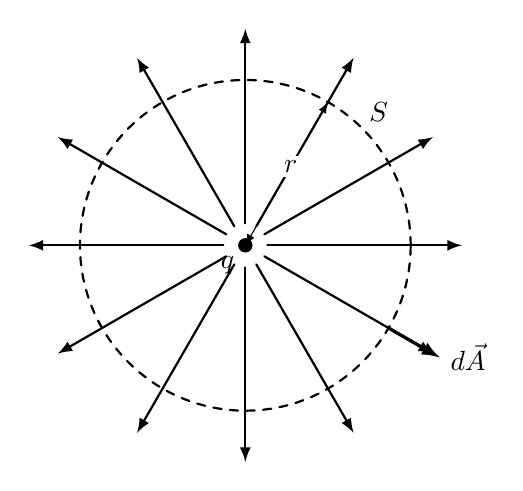
\begin{tikzpicture}[>=latex, line cap=round]

  % the Gaussian surface
  \draw[dashed, thick] (0,0) circle (2.1);
  \node[anchor=south west] at (1.45,1.45) {$S$};

  % the charge
  \fill (0,0) circle (2.6pt);
  % white backing so the label stays legible where the field lines converge
  \node[anchor=north east, fill=white, inner sep=1.5pt] at (-0.08,-0.08) {$q$};

  % radial field lines, drawn through the surface to show the flux
  \foreach \a in {0,30,...,330}{
    \draw[->, thick] (\a:0.28) -- (\a:2.75);
  }

  % the radius
  \draw[<->] (60:0) -- node[fill=white, inner sep=1.5pt, pos=0.55] {$r$} (60:2.1);

  % an area element
  \draw[->, very thick] (-30:2.1) -- ++(-30:0.75)
        node[anchor=west] {$d\vec{A}$};

\end{tikzpicture}
